% ====================================================================== %
%   author  :   louis tomczyk
%   date    :   2025-05-05
%   version :   2.1.0
% ====================================================================== %
%   ChangeLog
%   (1.0.0) - 2024.10.01    : création
%   (2.0.0) - 2024.12.12    : SEPARATOR, POEM - more than 2 poem family management
%                               + comments
%   (2.1.0) - 2025.05.05    : adendum for long poems
% ====================================================================== %

\def \Dagger{$^\dagger$}
\def \myPageBreak{
    \newpage
    \thispagestyle{empty}
    \mbox{} % Insère une boîte vide pour forcer une page blanche
    \newpage
}
\def \nothing{\textcolor{white}{.}}

\newcommand{\includeFiles}[2]{%
    \foreach \year in {#2} {%
        \input{Body/#1/\year_#1}
    }%
}



\newcommand{\separator}[1]{
    \begin{center}
    \ifnum\isPayant = 1
        \ifcase#1
            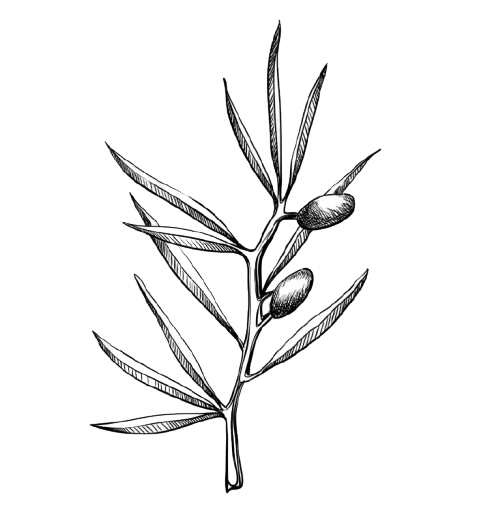
\includegraphics[width=0.5cm, angle=-90]{Figures/EaE/olivier.png} % Cas 0 : EaE
        \or
            
\includegraphics[width=0.5cm, angle=-90]{Figures/DHTH/acacia.png} % Cas 1 : DHTH
        \or
            
\includegraphics[width=0.25cm, angle=0]{Figures/tmp/ginko2.png} % Cas 2 : tmp
        \else
            \typeout{Erreur : Recueil non défini pour separator.}
            $\because$ % Symbole par défaut
        \fi
    \else
        $\star$ % Symbole par défaut pour les versions gratuites
    \fi
    \end{center}
}

% ========================================================================== %

\newcommand{\noteslist}{}
\newcommand{\addnote}[1]{%
    \gappto{\noteslist}{\item #1 \\} % Ajoute la note à la liste
}


% ========================================================================== %

\newcommand{\poem}[5]{% #1 date du poème, #2 titre, #3 \isPayant, #4 contenu, #5 addendum
    \begin{center}
        \vspace*{\fill}
        \begin{minipage}{0.8\linewidth}
            \begin{flushright}
                \ifnum\isPayant=1
                    \ifthenelse{\equal{#5}{}}{#1}{\textbf{#1}} \\
                \else
                    #1 \\
                \fi
                \ifnum\isPayant=1 #2 \\ \fi
            \end{flushright}
            \vspace{1 em}\par\noindent
            #4 % Contenu du poème
            \vspace{1 em}
            \separator{\poemIndex}
        \end{minipage}
        \vspace*{\fill}
    \end{center}

    \ifnum\isPayant=1
        \ifthenelse{\equal{#5}{}}{}{%
            \addnote{$\bm{#1}~\bullet$ #5}
        }%
    \fi
}

% ========================================================================== %





% ========================================================================== %

\newcommand{\poemBreakCover}[5]{ % poem on multiple pages: 1st page
\begin{center}
	\vspace*{\fill}
	    \begin{minipage}{0.8\linewidth}
		    \vspace{1em}
		    \begin{flushright}
			#1 \\  % Date
                \ifnum#3=1 #2 \\ \fi % Affiche le commentaire si #3 vaut 1
		    \end{flushright}
		    \vspace{1em}\par\noindent
		    #4
		    \vspace{1em}
	    \end{minipage}
	\vspace*{\fill}
    \end{center}
    
    \ifnum\isPayant=1
        \ifthenelse{\equal{#5}{}}{}{%
            \addnote{$\bm{#1}~\bullet$ #5}
        }%
    \fi
}

% ========================================================================== %

\newcommand{\poemBreakMiddle}[1]{ % poem on multiple pages: middle page
\begin{center}
	\vspace*{\fill}
	    \begin{minipage}{0.8\linewidth}
		    \vspace{1em}\par\noindent
                #1
		    \vspace{1em}
	    \end{minipage}
	\vspace*{\fill}
    \end{center}
}

% ========================================================================== %

\newcommand{\poemBreakEnd}[1]{ % poem on multiple pages: last page
\begin{center}
	\vspace*{\fill}
	    \begin{minipage}{0.8\linewidth}
		\vspace{1em}\par\noindent
            #1
		\vspace{1em}
            \separator{\poemIndex}
	    \end{minipage}
	\vspace*{\fill}
    \end{center}
}

% ========================================================================== %

\newcommand{\poemWO}[5]{% WithOut [separator]
    \begin{center}
        \vspace*{\fill}
        \begin{minipage}{0.8\linewidth}
            \begin{flushright}
                \ifnum\isPayant=1
                    \ifthenelse{\equal{#5}{}}{#1}{\textbf{#1}} \\
                \else
                    #1 \\
                \fi
                \ifnum\isPayant=1 #2 \\ \fi
            \end{flushright}
            \vspace{1 em}\par\noindent
            #4 % Contenu du poème
            \vspace{1 em}
        \end{minipage}
        \vspace*{\fill}
    \end{center}

    \ifnum\isPayant=1
        \ifthenelse{\equal{#5}{}}{}{%
            \addnote{\textbf{#1}~$\bullet$ #5}
        }%
    \fi
}

% ========================================================================== %

\newcommand\lastPage[1]{%
    \pagebreak
    \pagestyle{empty}
    \vspace*{\fill}
    \centering
    \ifnum\isPayant=1
        \ifcase#1
            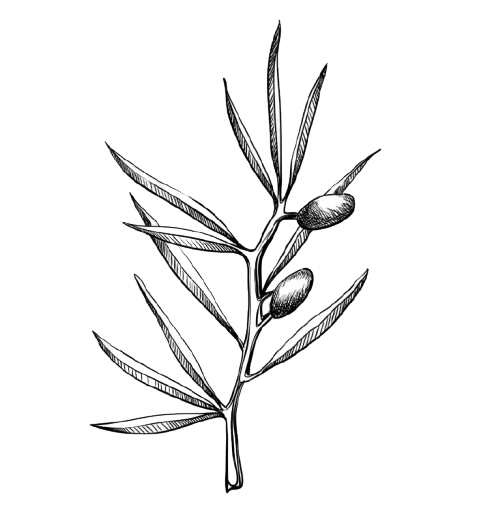
\includegraphics[width=0.5cm, angle=0]{Figures/EaE/olivier.png} % Cas 0 : EaE
        \or
            
\includegraphics[width=0.5cm, angle=0]{Figures/DHTH/acacia.png} % Cas 1 : DHTH
        \or
            
\includegraphics[width=0.5cm, angle=0]{Figures/tmp/ginko2.png} % Cas 2 : tmp
        \else
            \typeout{Erreur : Recueil non défini pour lastPage.}
            $\therefore$ % Symbole par défaut
        \fi

		~\par
    
	    \href{https://www.vers-sans-blason.fr/}{www.vers-sans-blason.fr}
    \else
        \centering
        
\includegraphics[width=2cm]{Figures/qr_code.png} % QR code pour la version gratuite
		~\par
		
		\href{https://www.vers-sans-blason.fr/}{www.vers-sans-blason.fr}
	\fi
    
    \vspace*{\fill}
}
